% !TeX root = ../main.tex

\chapter{Numerical modelling method}

Since the subduction process contain slow deformation and the constrain for deep lithosphere evolution is not well understand from either geophysical observation in depth or geology study in time, computer model is a suitable way to  study subduction zone, especially the numerical model. While the analytic solution is hard to solve, numerical model has become a useful method for studying Earth evolution. 

The numerical models in this study address the dynamics process of flat subduction, in which an oceanic plate subducts beneath continental plate. The goal of this work is to address the controls on subducting plate dynamics and to determine the conditions under which flat subduction may develop. 

In this chapter, we introduce the method of numerical model and the initial model setup. In section 2.1, we discuss the governing equations. In section 2.2, the finite elements method will be briefly discuss. In section 2.3, we introduce the Fast Lagrangian Analysis of Continua technique. In section 2.4, the model geometry is presented. The material properties, phase transition and model boundary conditions are given in section 2.5 ,2.6 and 2.7, respectively.

\section{Governing equation}

\subsection{Continuum---Conservation of mass}

In geodynamics modelling, we consider major rock units as continuous geological media. The continuous description is described by field variables such as density, pressure, velocity, strain, etc. 
The continuity can be transformed into quantitative mathenatical formalism, that is, continuity equation.

The mass conservation equation in Lagrangian form is as follow
\begin{align}
\frac{\partial \sigma_{ij}}{\partial x_j}+\rho g_i = \rho \frac{\partial D_{vi}}{\partial t} 
\end{align}
A Lagrangian points is strictly connected to a single material point and is moving with this point. Therefore, the same material point is always in same coordinate independent of the moment of time. On the other hand, Eulerian point is an immobile point.
The proof of eq.(2.1) is as follow
\begin{figure*}[ht!]
    \centering
    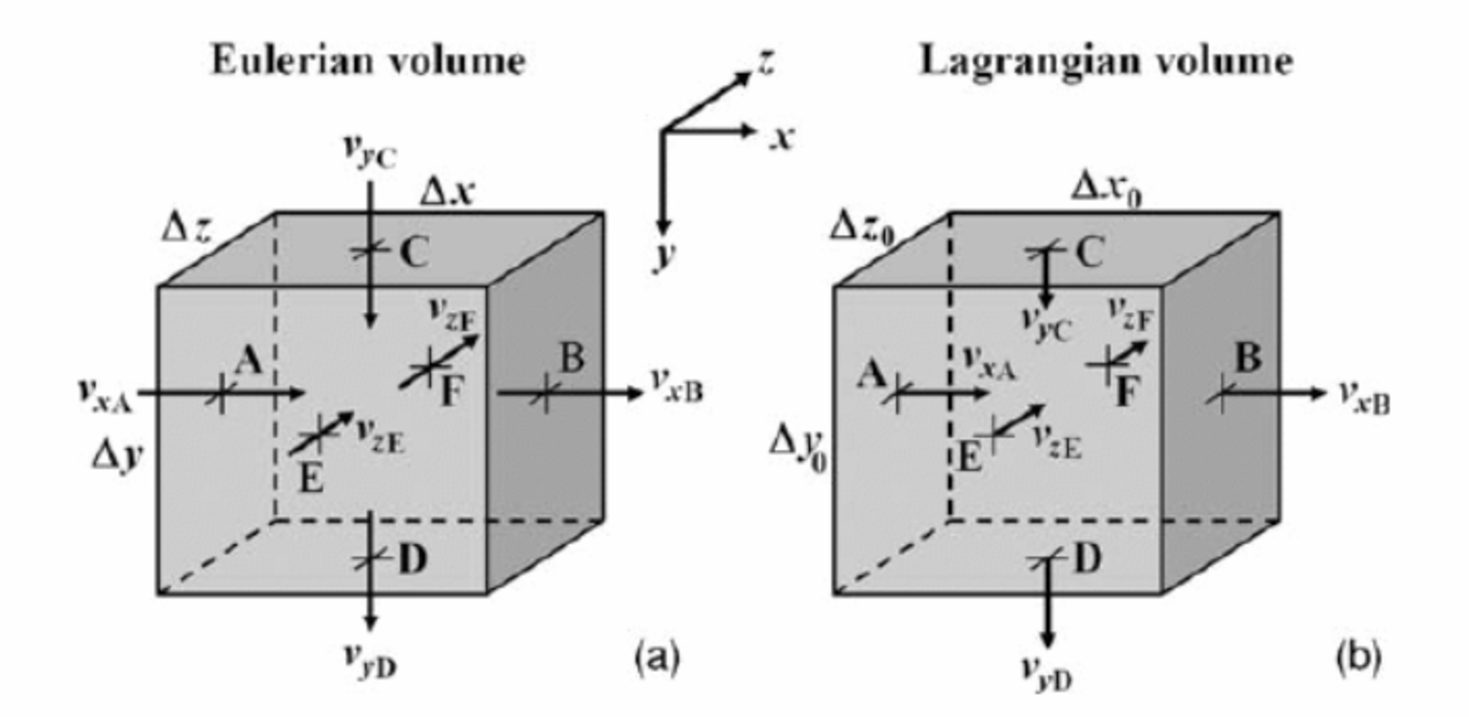
\includegraphics[width=4.5in]{eulerian_and_lagrangian.pdf}
    \caption{ Eulerian (a) and Lagrangian (b) elementary volumes considered for the derivation of continuity equation. }
    \label{fig::Lagrangian Volume}
\end{figure*}
 
Since the volume is always related to the same material points, the amount of mass in the moving Lagrangian volume remains constant. However, the volume change due to the internal expansion or contraction process. The initial average density $\rho_0$ in a Lagrangian volume ($V_0$) is given by:
\begin{align}
\rho_0 = \frac{m}{\Delta x_0 \Delta y_0 \Delta z_0}
\end{align}
After a small period of time ($\Delta t$), the Lagrangian volume undergo internal process, thus the volume become $V_1$ and the average density change to:
\begin{align}
\rho_1 = \frac{m}{\Delta x_1 \Delta y_1 \Delta z_1}
\end{align}

Lagrangian material in time derivative is:
\begin{align}
\frac{D\rho}{Dt} \approx \frac{\Delta \rho}{\Delta t} = \frac{\rho_1-\rho_0}{\Delta t}=\frac{m}{\Delta x_1 \Delta y_1 \Delta z_1\Delta t}-\frac{m}{\Delta x_0 \Delta y_0 \Delta z_0\Delta t}
\end{align}
The relationship between new and old dimensions of Lagrangian volume is base on the relative movements of the volume's boundary, the displacement is equal to the velocity times duration period:
\begin{align}
\Delta x_1 = \Delta x_0+\Delta t\Delta v_x\\
\Delta y_1 = \Delta y_0+\Delta t\Delta v_y\\
\Delta z_1 = \Delta z_0+\Delta t\Delta v_z
\end{align}
By using the equation above (2.5-2.7), replace the $\Delta x_1$, $\Delta y_1$, $\Delta z_1$ to eq 2.4:
\begin{align}
\frac{D\rho}{Dt} \approx \frac{\Delta \rho}{\Delta t} =\frac{m\Delta x_0 \Delta y_0 \Delta z_0-m\Delta x_1 \Delta y_1 \Delta z_1}{\Delta x_1 \Delta y_1 \Delta z_1\Delta t\Delta x_0 \Delta y_0 \Delta z_0}
\end{align}
Since $\Delta x_0 \Delta y_0 \Delta z_0=\rho_0$, the following expression can be obtain:
\begin{align}
\frac{\Delta \rho}{\Delta t}+\rho_0\frac{\frac{\Delta v_x}{\Delta x_0}+\frac{\Delta v_y}{\Delta y_0}+\frac{\Delta v_z}{\Delta z_0}+K_1}{K_2} = 0
\end{align}
\begin{align}
K_1 = \Delta t(\frac{\Delta v_x}{\Delta x_0}\frac{\Delta v_y}{\Delta y_0}+\frac{\Delta v_x}{\Delta x_0}\frac{\Delta v_z}{\Delta z_0}+\frac{\Delta v_y}{\Delta y_0}\frac{\Delta v_z}{\Delta z_0}+\Delta t \frac{\Delta v_x}{\Delta x_0}\frac{\Delta v_y}{\Delta y_0}\frac{\Delta v_z}{\Delta z_0})
\end{align}
\begin{align}
K_2=(1+\Delta t\frac{\Delta v_x}{\Delta x_0})(1+\Delta t\frac{\Delta v_y}{\Delta y_0})(1+\Delta t\frac{\Delta v_z}{\Delta z_0})
\end{align}
where $K_1$ and $K_2$ are coefficients which respectively tend to zero and unity when $\Delta t$ tends to zero. Eq (2.9) can be rewrite to:
\begin{align}
\frac{D\rho}{Dt}+\rho\frac{\partial v_x}{\partial x}+\rho\frac{\partial v_y}{\partial y}+\rho\frac{\partial v_z}{\partial z} = 0
\end{align}
or
\begin{align}
\frac{D\rho}{Dt}+\rho div(\vec v) = 0
\end{align}

While in geodynamics modelling, the density variations are small enough to be ignored, which is the result of Boussinesq approximation. The Boussinesq approximation assume that the density is linear proportional to the temperature and the small density variation is then neglected, except the gravity term.
\begin{align}
\rho (T) = \rho_0[1-\alpha (T-T_0)] 
\end{align}
where $\rho_0$ is the reference density at temperature $T_0$ and $\alpha$ is the volumetric thermal expansion coefficient. The boussinesq approximation also represent the incompressible condition, which mean the density of material points does no change with time. The incompressible continuity equation is broadly used in numerical geodynamic modelling, although on many cases it is rather big simplification. 
\begin{align}
\nabla \cdot (\vec v) = 0 
\end{align}
Eq. (2.15) is the conservation of mass in our numerical modelling approach.

\subsection{Motion---Conservation of momentum}
In geodynamics, the time-dependent phenomena involve deformation of continuous media, which is the effect of the balance of internal and external forces that act in these media. So as to relate forces and deformation, an equation of motion may be used --The momentum equation. The momentum equation is a differential equivalent of Newton’s second law to a continuous medium.
\begin{align}
f=ma
\end{align}
$f$ is the net force acting on the object and $m$ is the mass of material. The momentum equation for a continuous medium in the gravity field:
Eulerian Form:  \begin{align}
\frac{\partial \sigma_{ij}}{\partial x_j}+\rho g_i = \rho (\frac{\partial v_i}{\partial t}+v_j\frac{\partial v_i}{\partial x_j})
\end{align}
Lagrangian Form:  \begin{align}
\frac{\partial \sigma_{ij}}{\partial x_j}+\rho g_i = \rho \frac{\partial D_{vi}}{\partial t}
\end{align}
\begin{figure*}[ht!]
    \centering
    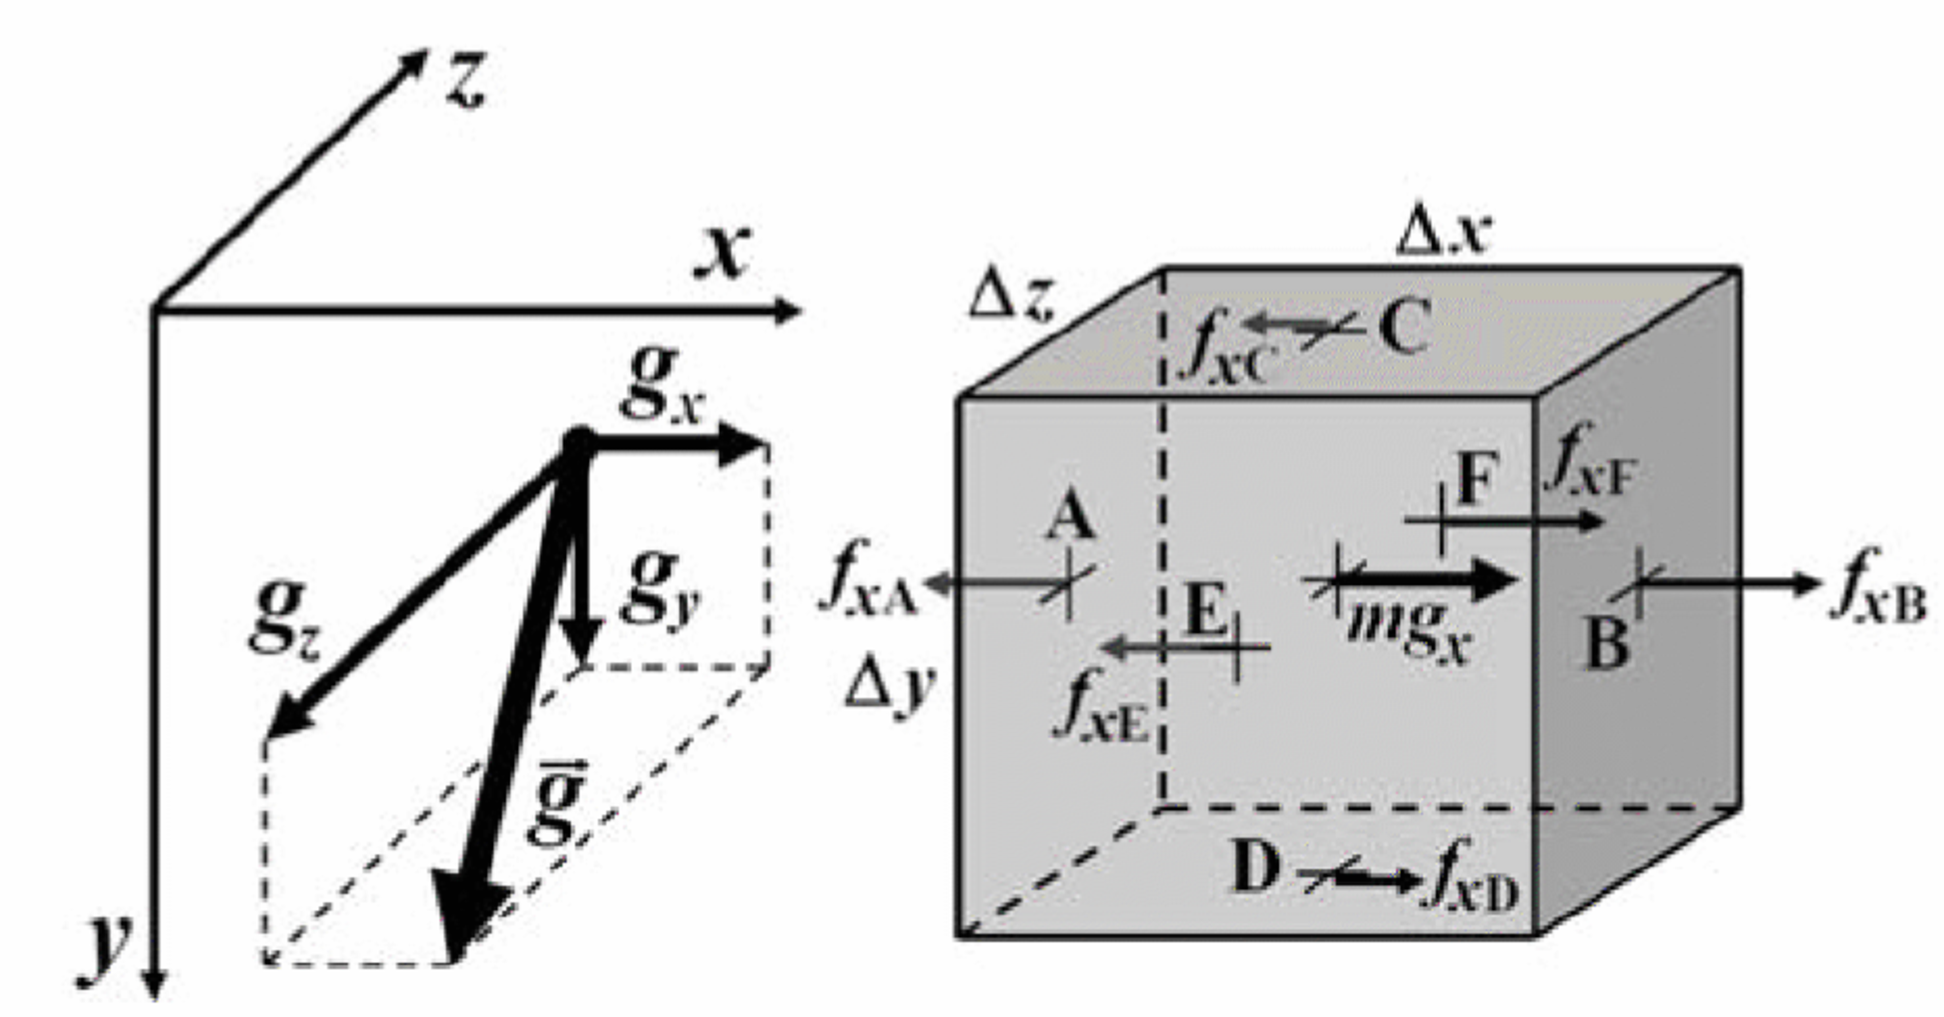
\includegraphics[width=4in]{momentum.pdf}
    \caption{ Lagrangian elementary Volume considered for the derivation of the respective form of x-momentum equation.}
    \label{fig::Lagrangian Volume}
\end{figure*}

While considering a small Lagrangian volume, the net force acting on the object which can be computed locally. We will proof the momentum equation of Lagrangian Form below:

For x-component
\begin{align}
f_x=f_{xA}+f_{xB}+f_{xC}+f_{xD}+f_{xE}+f_{xF}+mg_x 
\end{align}
$f_{xA}- f_{xF}$ are stress-related forces, from the outside of the volume on the respective boundaries A-F. 
$f_g=m_gx$ is the gravity force.
\begin{align}
f_{xA} = -\sigma_{xxA}\Delta y\Delta z\\
f_{xB} = +\sigma_{xxB}\Delta y\Delta z\\
f_{xC} = -\sigma_{xyC}\Delta x\Delta z\\
f_{xD} = +\sigma_{xyD}\Delta x\Delta z\\
f_{xE} = -\sigma_{xzE}\Delta x\Delta y\\
f_{xF} = +\sigma_{xzF}\Delta x\Delta y
\end{align}
We replace the force Eq(2.20-2.25) to Eq (2.19):
\begin{align}
(\sigma_{xxB}-\sigma_{xxA})\Delta y\Delta z+(\sigma_{xyD}-\sigma_{xyC})\Delta x\Delta z+(\sigma_{xzF}-\sigma_{xzE})\Delta x\Delta y+mg_x = ma_x 
\end{align}
Normalising both sides by considered Lagrangian volume
\begin{align}
V=\Delta x\Delta y\Delta z
\end{align}
we obtain
\begin{align}
\frac{(\sigma_{xxB}-\sigma_{xxA})\Delta y\Delta z}{V}+\frac{(\sigma_{xyD}-\sigma_{xyC})\Delta x\Delta z}{V}+\frac{(\sigma_{xzF}-\sigma_{xzE})\Delta x\Delta y}{V}+\frac{m}{V}g_x=\frac{m}{V}a_x
\end{align}
or
\begin{align}
\frac{\Delta\sigma_{xx}}{\Delta x}+\frac{\Delta\sigma_{xy}}{\Delta y}+\frac{\Delta\sigma_{xz}}{\Delta z}+\rho g_x = \rho a_x
\end{align}
While the differences of the respective stresses components all tend to zero, we obtain:
\begin{align}
\frac{\partial\sigma_{xx}}{\partial x}+\frac{\partial\sigma_{xy}}{\partial y}+\frac{\partial\sigma_{xz}}{\partial z}+\rho g_x = \rho a_x
\end{align}
or 
\begin{align}
\partial_j\sigma_{ij}+\rho g_i = \rho \ddot u
\end{align}
where $u$ is the displacement.
\subsection{Heat equation --- Conservation of energy}

To describe the balance of energy in a continuum material, heat equation is apply to measure the temperature change. The heat equation sloved the heat transport and porvided the temperature field. Below is the heat equation in Lagrangian form :
\begin{align}
\rho C_p \frac{DT}{Dt} = -\frac{\partial q_x}{\partial x}-\frac{\partial q_y}{\partial y}-\frac{\partial q_z}{\partial z}+H_s+H_L
\end{align}

where $\rho$ is the density, $C_p$ is the heat capacity at constant pressure (isobaric heat capacity), $H_s$ is shear heating and $H_L$ is the latent heat production.

The proof of heat equation is show below:

(加上heat equation的推倒
加圖)

Base on the Boussinesq approximation, the imcompressible Lagrangian form governing equations are:
\begin{align}
\nabla \cdot (\vec v) = 0 
\frac{\partial \sigma_{ij}}{\partial x_j}+\rho g_i = \rho \frac{\partial D_{vi}}{\partial t}
\rho C_p \frac{DT}{Dt} = -\frac{\partial q_x}{\partial x}-\frac{\partial q_y}{\partial y}-\frac{\partial q_z}{\partial z}+H_s+H_L
\end{align}

Describe conservation of mass, conservation of momentum and conservation of energy, respectively.


\section{Finite elements method}

finite elements method

\section{Rheological behavior}

**What is viscous and the viscous rheology of rock**

In the near-surface region, rocks undergo relatively low temperature and, therefore, the Earth's lithosphere easily result in brittle (at low pressure) and plastic (at high pressure) deformation. 
While in the deep earth, temperature increasing with depth, rocks behave viscous with irreversible deformation. 
Therefore, if a geodynamics model need to account for a wide range of rocks properties, it should consider the elasto-visco-plastic rheology of rocks.

Elastic rheology assume that the relationship between applied stress and strain is proportionality. 

\begin{figure*}[ht!]
    \centering
    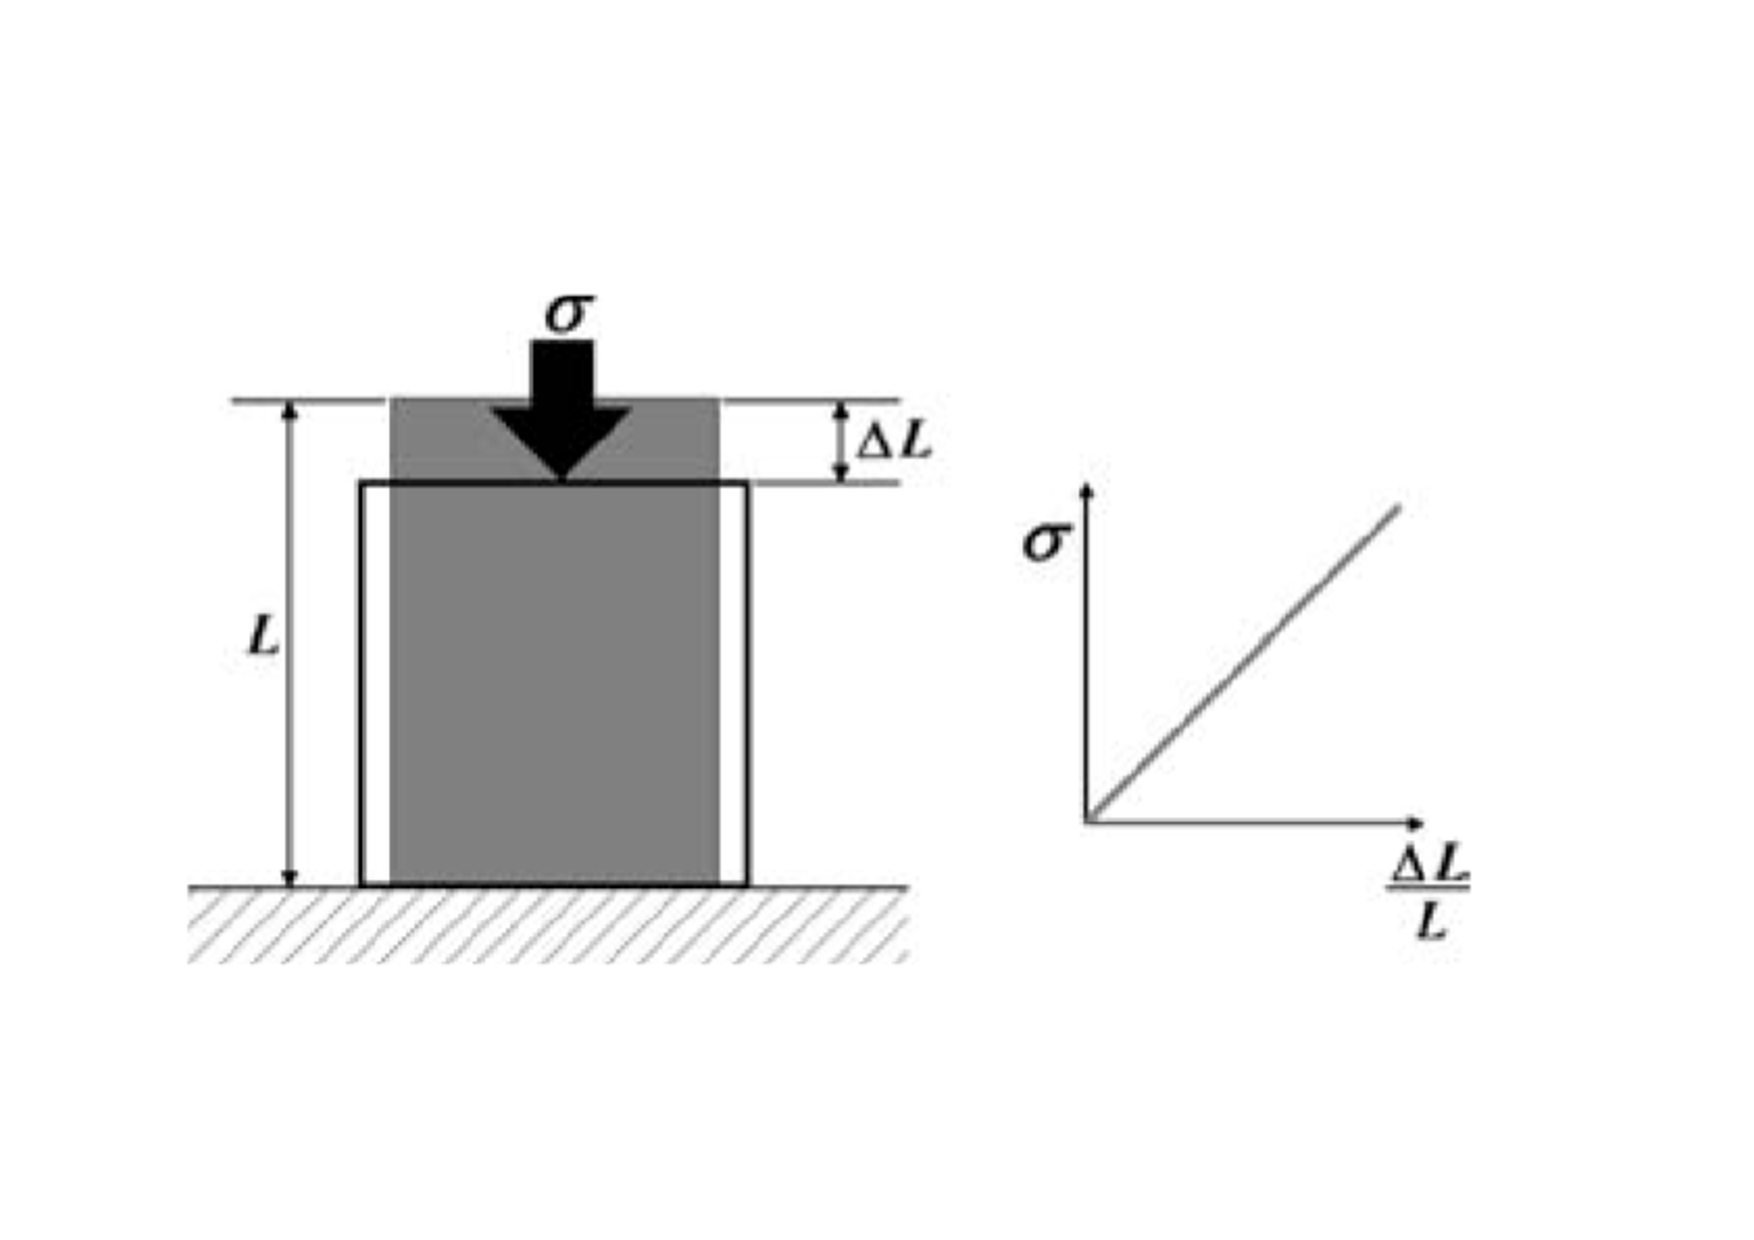
\includegraphics[width=3in]{elasticdeformaiton.pdf}
    \caption{ Elastic deformation  }
    \label{fig::elastic}
\end{figure*}

While plastic.......


Viscous rheology define....

\section{Phase change}

In this study, we use markers to trace the rocks phases, pressure and temperature. 
At the time the pressure and temperature satisfy the phase transformation condition, the marker will turns to new rock phase. 
A basalt element represent an element with more than 30 presents of the basalt phase markers. 
In this case, the element behave the deformation as same as the basalt rheology.

\subsection{Peridotite --- Serpentinite}

Once the subducting plate sink into mantle, sediment on oceanic plate undergo higher pressure and temperature that release a large amount of fluids. 
On the other hand, the oceanic plate itself also carries seawater into the mantle. 
Fluids in subduction zone mostly concentrated in the mantle wedge. 
The dry mantle wedge undergo hydration process, lead to the transformation of peridotite to serpentinite.  
The serpentinite depth and thickness in subduction zone is not well understand since the seismic study constrain still contain high uncertainly, we model the phase transformation process of serpentinite in parameter way.     

Serpentinite are stable in the colder mantle wedge relative to deeper mantle, and therefore once the serpentinite under unstable field, we assume that serpentinite rocks release fluid and transfer to peridotite. 
The following equations are the conditional expressions of serpentinite---peridotite transformation. Figure is the phase diagram of mantle phases.


\subsection{Basalt --- Eclogite}

As the oceanic crust sink into deeper mantle, the mafic rocks enters the eclogite stability field in the condition of high pressure. 
Therefore, basalt phases transform to eclogite.  
In this model, oceanic crust are tracked and compared with the eclogite stability filed, the following equations are the conditional expressions of mafic rocks transformation. 
Figure below is the mafic rocks phase diagram.
\begin{figure*}[ht!]
    \centering
    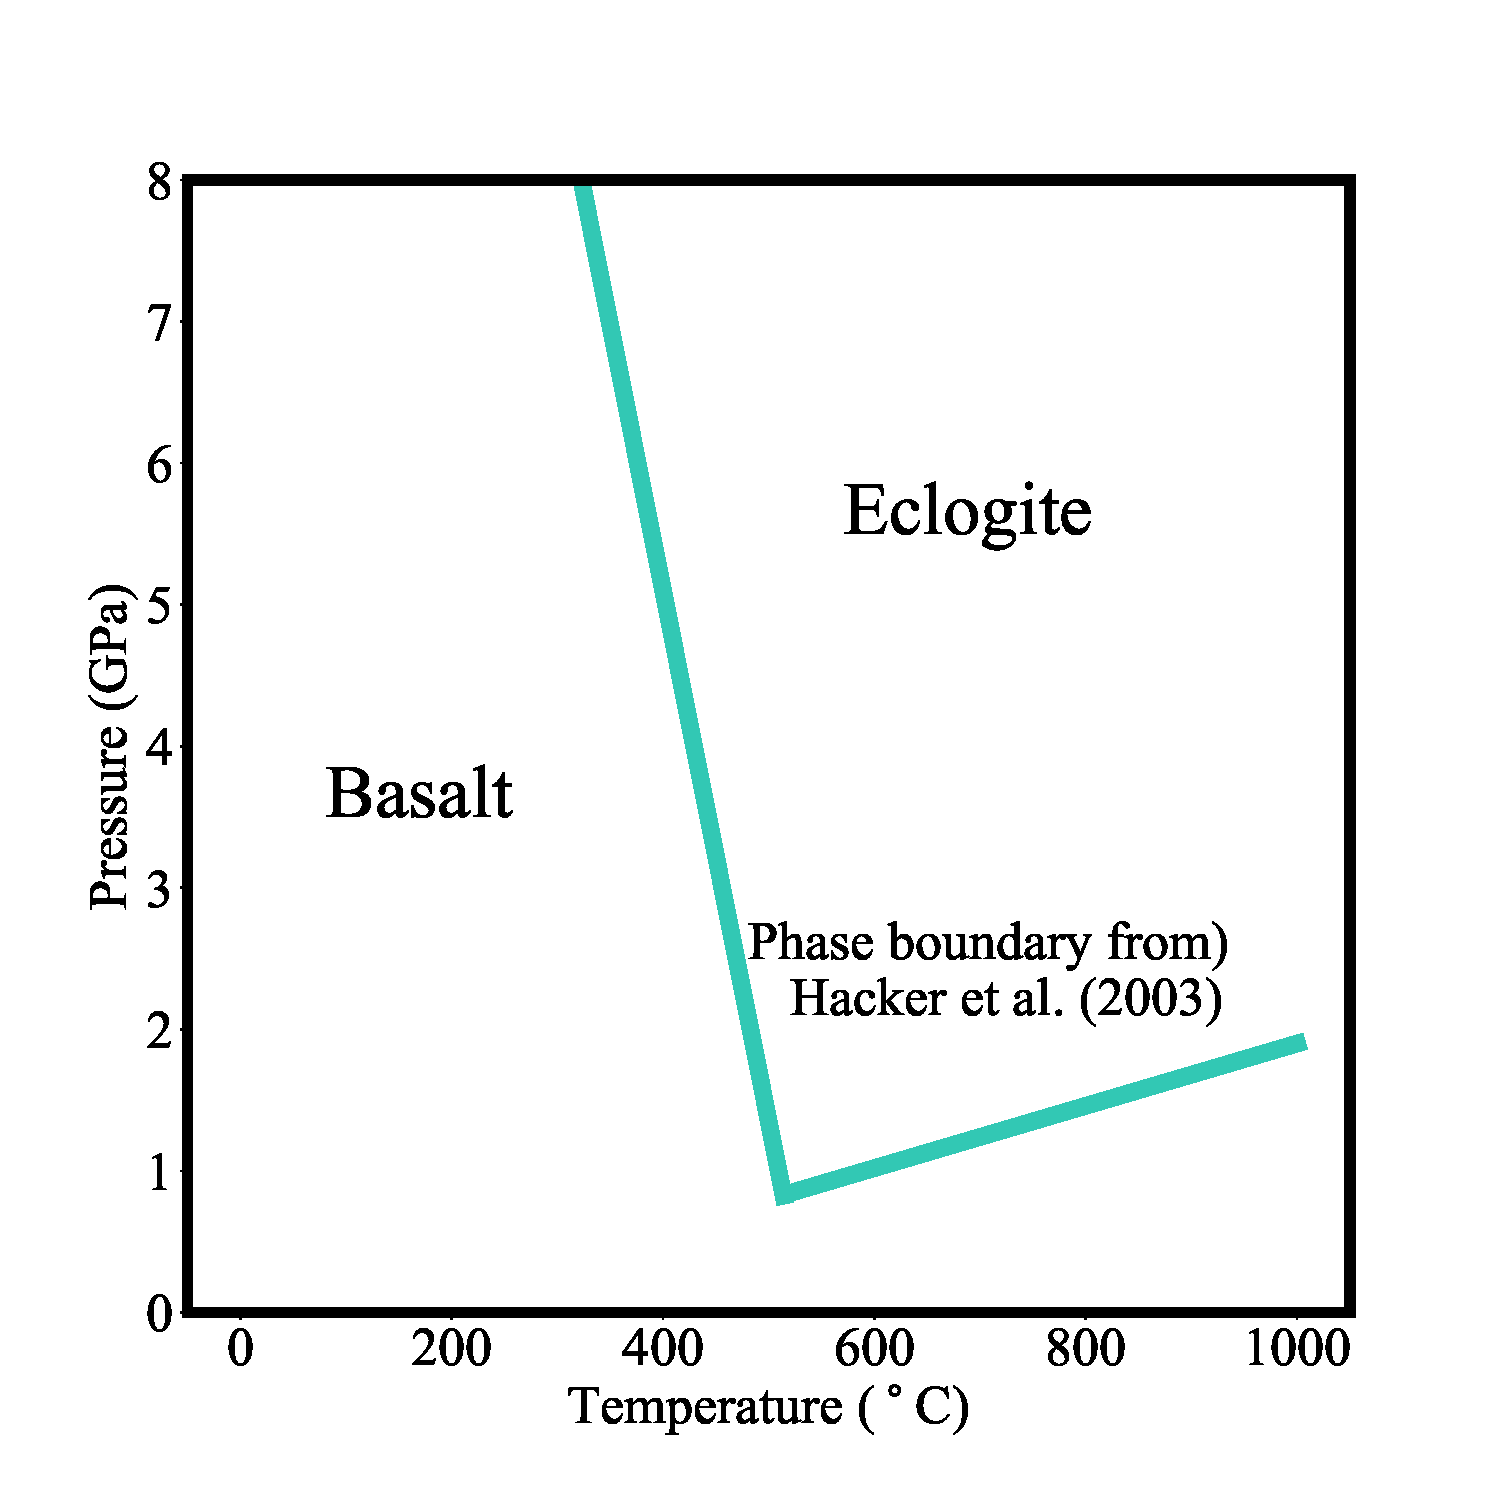
\includegraphics[width=3in]{basalt_phase_diagram.pdf}
    \caption{ Phase diagram showing the stability field for mafic rocks (Hacker et al., 2003).  }
    \label{fig::elastic}
\end{figure*}

\subsection{Sediment --- Schist}

Once sediment undergo higher pressure, the compression process and mataphase(變質作用)process occur.
In this model, the following equations are the conditional expressions of transformation process of sediment to schist.

$T > 650^{\circ} C$\\
$depth >  20 $km 

The subducted sediments will turn into schist when temperature is greater than 650$^\circ$C and pressure is greater than (一個數字 算出來?)

\subsection{Hydrated olivine --- Peridotite}

We considering a hydrated peridotite under the oceanic crust in our model. 
The magma will only generated above the hydrated subducting oceanic lithosphere.
Once the tempertaure is too high to make the rock contain water, the hydrated olivine transform to normal perodotite.
The following equation is the conditional expression of this transgformation.

$T > 800-35\times 10^{-9}\times (depth-62)^{2\circ}C$

\section{Boundary condition}

\subsection{Kinematic boundary condition}

\subsection{Thermal boundary condition}

For oceanic lithosphere, we used half space cooling model in our model to defined the thermal condition. 
The plate depth is proportional to the square root of oceanic lithosphere age, and therefore, the half space cooling model can predict will for the temperature of the oceanic plate.
Follow by David and Lister,1974:

$T=T_m\cdot {erf}(\frac{z}{2\sqrt{\kappa t}})$

$T$ is the temperature, $T_m$ is the mantle temperature, in this model the temperature is 1330,
$z$ is the depth from surface and $\kappa$ is the thermal conductivity ceoficient, that is, $10^{-6}$ in this study.
$t$ is the lithosphere age in Myr.


For continental lithosphere, the thermal condition is defined in linearly.


\section{FLAC}

We used the Fast Lagrangian Analysis of Continua (FLAC) technique. FLAC is a two-dimensional, explicit finite element with Lagrangian gird of numerical program.  

\section{Initial Model}

initial model


